\documentclass{article}
\usepackage[utf8]{inputenc}
\usepackage[left=3cm,top=2cm,right=3cm,bottom=3cm,nohead]{geometry}
\usepackage{enumitem}
\usepackage{amsmath}
\usepackage{amssymb}
\usepackage{amstext}
\usepackage{subfig}
\usepackage{url}
\usepackage{comment}
\setlength\parindent{0pt}
\usepackage{calligra}
\usepackage{todonotes}
\usepackage{siunitx}
\usepackage{wasysym}
\usepackage{hyperref}
\usepackage{tcolorbox}

\usepackage[justification=centering]{caption}
%\captionsetup[figure]{labelfont=bf} %makes 'Figure' bold 
\setlength{\parindent}{0pt}


% Bouke commands
\newcommand\numberthis{\addtocounter{equation}{1}\tag{\theequation}}
\newcommand{\unit}[1]{\ensuremath{\, \mathrm{#1}}}
\newcommand{\aap}{A\&A}
\newcommand{\nat}{Nature}
\newcommand{\araa}{Annual Review of Astronomy and Astrophysics}
\newcommand{\mnras}{Monthly Notices of the Royal Astronomical Society}
\newcommand{\pasj}{Publications of the Astronomical Society of Japan}
\newcommand{\apj}{The Astrophysical Journal}
\newcommand{\apjl}{The Astrophysical Journal Letters}
\newcommand{\apss}{Astrophysics and Space Science}
\newcommand{\pasp}{Publications of the Astronomical Society of the Pacific}
\newcommand{\bain}{Bulletin Astronomical Institute of the Netherlands}


\title{\textbf{HEA comptonization project - Blazar 3C454.3 }}
\author{Bouke Jung (11857269)}
\date{June 8, 2018}

\begin{document} 

\maketitle
\tableofcontents

\abstract{The following report contains a brief overview of a Monte Carlo code written in the context of the UvA course \textit{High Energy Astrophysics: Radiative Processes and Relativistic Flows}. The code can be used to generate spectra of astrophysical objects which exhibit inverse Compton scattering of black body photons in a highly relativistic jet. Several techniques are discussed for sampling photon and electron energies from black body and power-law distributions. Resulting spectra are compared to SED data of the blazar 3C454.3 for verification. Although the program is not able to reproduce the entire SED of this source (particularly below $10^{15}$ Hz and above $10^{20}$ Hz, some important spectral features are rederived with relative success (in particular the general spectral shape associated with the inverse compton scattering processes and the SED magnitude between $10^{18}$ and $10^{20}$ Hz).}

\newpage

\section{Introduction}
    Constituting highly versatile and powerful modeling techniques, Monte Carlo simulations have developed into one of the principal tools for tackling computational problems in physics and astrophysics over the past decades. Its applications can be found in a diverse range of subjects, such as the study of ion transport phenomena \cite{Haggmark1980}, quantum dots \cite{Gull2011} and neutrino events \cite{Andreopoulos2010}. This report, however, presents a Monte Carlo code written in the context of astrophysical compton scattering. Following the work of Pozdnyakov, Sobol and Syunyaev\cite{Pozdnyakov1983}, as well as Carter and Cashwell \cite{Carter1975}, a model has been set up which enables one to produce spectral energy density (SED) profiles for objects which exhibit compton scattering of thermally produced photons in a highly relativistic jet. To verify that the model functions correctly, we attempted to reproduce the SED of the blazar 3C454.3. This object is particularly interesting since it forms one of the main sources for ultra-high energy gamma-rays in the local universe. To start off the report, we'll explain what algorithms were used to obtain flux density values for 3C454.3. By comparing the spectrum generated by the code to flux densities found in the literature, we will subsequently evaluate the validity of our model. The report will be concluded with a discussion of any remaining discrepancies and complications as well as potential improvements.


\section{The compton scattering algorithm}
    Similar to other areas of (astro)physics where the method is frequently used, studying compton-induced SEDs via Monte Carlo simulations often proves fruitful because of the highly coupled nature of the underlying physical processes. By randomly sampling a large number of photons from an appropriate initial distribution and by applying the various formulae and operations associated with (inverse) compton scattering to these photons, it is possible to rederive the deterministic spectra of high-energy astrophysical sources via essentially indeterminate input. This section is devoted towards explaining the various components that comprise the Monte Carlo code we used to generate the SED of a source like 3C454.3. We'll start with a discussion of the various sampling methods that were used, after which we'll present the operations subsequently applied to execute the scattering of each photon.

    \subsection{Sampling methods}
        Constituting perhaps the most defining aspect in any Monte Carlo simulation, it is quintessential that we properly address the random sampling algorithms that were used in order to derive our spectra. As mentioned in the introduction, our code specializes in generating spectra created by inverse Compton scattering of black body radiation. Our input spectrum will therefore have to consist of photons drawn from a Planck spectrum. There are different methods which allow sampling from a black body spectrum. One particularly fast algorithm uses a clever approximation \cite{Carter1975, Pozdnyakov1983}. Denoting the normalized black body distribution by $b_\nu$ we can write:
    
            \begin{equation}
                b_\nu = \frac{15}{\pi^4} \frac{x^3}{e^x - 1}
            \end{equation} \label{eq:BB}

        where $\nu = (k_B T / h) x$ is the photon frequency. Expanding the term $1/(e^x -1)$ we can rewrite this as:

            \begin{equation}
                b_\nu = \frac{15}{\pi^4} \sum_{m=1}^{\infty} m^{-3} b_{\nu,m}
            \end{equation}
        
        where the functions $b_{\nu,m} = m^3 x^3 e^{-xm}$ are conform to Gamma distributions. To sample from these distributions, we draw five random numbers $\xi_i$ ($i\in{0,1,2,3,4}$) from a uniform distribution between 0 and 1 and compute the value:
        
            \begin{equation}
                L = \mathrm{min}\left( l, \sum_{j=1}^l j^{-4} \geq \xi_0 \frac{\pi^4}{90}\right)
            \end{equation}
        
        From this quantity the random photon frequency can be computed as:

            \begin{align*}
                x &= -L^{-1} \sum_{i=1}^4 \ln(\xi_i) \\
                \longrightarrow \nu &= \frac{k_B T}{h} x
            \end{align*}

        Once an initial photon frequency is selected, the next operations in our model will consist of several Lorentz boosts to transform to the electron rest frame. Since our model assumes a geometry where the initially generated black body photons (originating from a dusty torus surrounding an AGN in the case of 3C454.3) undergo inverse compton scattering with electrons in a nearby relativistic jet, we will first have to transform to the jet rest frame. This can be accomplished using the famous relativistic boost transformation:
        
            \begin{equation}
                E' = E \Gamma (1 - \beta \cos(\alpha))
            \end{equation} \label{eq:transfE}

        where $\Gamma = 1/(1-\beta^2)$ represents the jet Lorentz bulk factor and where $\alpha$ denotes the angle between the initial photon propagation direction and the jet. 
        
        \par Before determining whether the photon undergoes inverse compton scattering or not, we first select a random potential scattering electron, by sampling a velocity $\beta = \sqrt{1 - 1/\gamma^2}$ from an inverse power-law distribution $p(E) \propto E^{-p}$. The result is used to draw a random scattering incident angle $\mu$ from $f(\mu) = (1 - \beta \mu) / 2$, completing the creation of the potential scattering electron. We use different sampling methods for deriving both quantities. \\
        The electron velocity is most easily generated using a method called \textit{inverse transform sampling}. Since the cumulative distribution function (CDF) of a normalized distribution function f is always bound between 0 and 1, we can substitute a randomly drawn number between these values into the inverse CDF (also called the quantile function) in order to sample from f. In case of an inverse power-law distribution, this yields the equation:

            \begin{equation}
                E = (1-\xi)^{\frac{1}{1-p}}
            \end{equation}

        where $\xi \in [0,1]$ denotes the randomly drawn CDF value and where $p$ stands for the power-law index. \\
        In case of the distribution $f(\mu) = (1 - \beta \mu) / 2$ it's simpler to use a method called \textit{rejection sampling}\footnote{The quantile function of this distribution will contain a square root dependence which leads to complications when using the inverse sampling method if the random argument under the square root becomes negative.}. This method is in many ways akin to throwing darts, in the sense that we draw a random point (i.e. an x- and a y-value), throw it at the distribution function and determine whether it lies below or above the distribution curve. In case of the latter, the point is rejected and a new point is drawn, whereas for the former case, the point is accepted and inputed into the remainder of the program. \\

        
        
        \subsection{The inverse Compton scattering}

        \par Once a random photon and a random electron have been generated, the program has to decide whether compton scattering takes place or not. To do so we use the simple criterion that scattering will occur as long as $\xi \geq P$ for $\xi$ another random draw from a uniform distribution $unif(0,1)$ and with P given by:

            \begin{align*}
                P &= \begin{cases}
                        \frac{1}{2} \frac{E_\gamma}{eV}, & E_\gamma > 1 eV \\
                        \frac{1}{2}, & E_\gamma \leq 1 eV
                     \end{cases}
            \end{align*}
        
        In case the criterion is met, the actual scattering will be conducted via the usual formulae for inverse compton scattering (see e.g. Rybicki and Lightman (1979) \cite{Rybicki1979}). The photon is first boosted to the rest frame of the electron, after which the new photon energy is computed via:

            \begin{equation}
                \epsilon_1' = \frac{\epsilon'}{1+\frac{\epsilon'}{mc^2}(1-\cos\theta)}
            \end{equation}
         
        The observed photon energy is provided by performing a Lorentz boost twice: first we transform back to the jet rest frame, after which we transform to the observer frame using \ref{eq:transfE} where, this time, $\alpha$ denotes the angle between the jet and the angle of observation. \\
        The final step of the Monte Carlo code consists of dividing the photon energy range resulting from the above operations into sensible energy bins and adding each individual simulated photon correspondingly. As mentioned in Pozdnyakov et al. (1983) \cite{Pozdnyakov1983} (see the last paragraph in particular), normalizing the resulting counts by the total number of simulated photons, yields a spectrum that is directly proportional to the flux $F_\nu / h\nu$. Hence, an SED can be computed from the randomly sampled photons by multiplying the final counts in each bin with the corresponding bin energy. 


 


\section{Results for 3C454.3}

    \begin{figure}[ht]
        \centering
        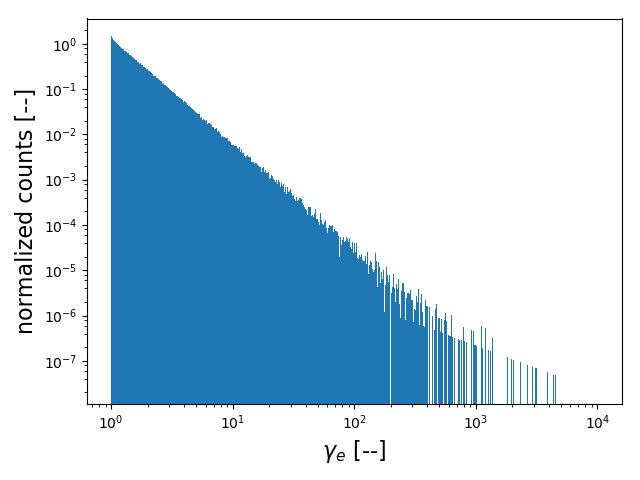
\includegraphics[width=0.9\textwidth]{3C454_3_electrondist.png}
        \caption{The normalized electron distribution used to randomly draw electrons for inverse compton scattering.}
    \end{figure}
    \label{fig:electron_distr}

    Having explained the general theory behind the Monte Carlo procedures of our code as well as the compton scattering criteria, we can move on to several results found using our model. An interesting source which the model can be applied to is the blazar 3C454.3. Surrounded by a dusty torus of gas at a few hundred kelvin, the blazar provides a background field of black body distributed photons, complying very well with the input spectrum assumed in our code. Furthermore, the source exhibits a highly relativistic jet with a bulk gammma factor somewhere between 10 and 20 \cite{Hovatta2009,Gupta2017}, allowing for efficient inverse compton scattering, which is ideal to test our model. Before we can discuss the SED found using the Monte Carlo simulation, we'll first have to discuss the source-specific parameters which we gave to our program as input. \\

    \par To generate the background flux of Planckian photons originating from the dusty torus, we need to input the temperature of the comprising gas $T$. Judging from spectra such as the ones given in Sikore et al. (2008) \cite{Sikora2008} and Gupta et al. (2017) \cite{Gupta2017}, which display a cut-off around $10^{13.3}$ Hz, and assuming that this cut-off roughly coincides with the peak of the dusty torus black body spectrum, we find via Wien's displacement law that:

        \begin{align*}
            T &\approx \frac{1}{\alpha} \frac{h \nu_{max}}{k_B T} \\
              &\approx \frac{10^{13.3}}{5.879\cdot 10^{10}} K \\
              &\approx 340 K
        \end{align*}

    \begin{figure}[p]
        \centering
        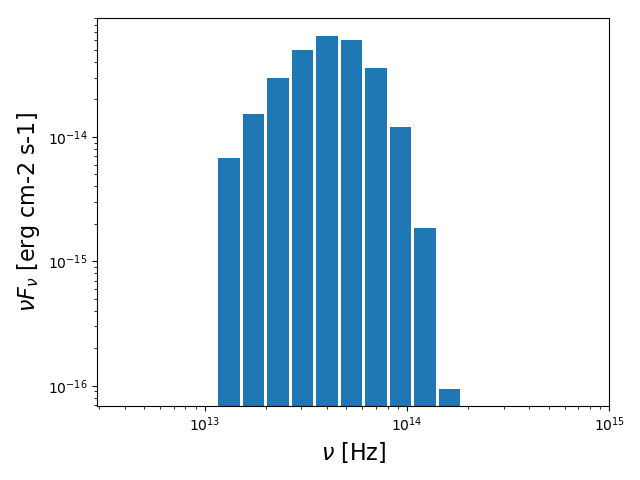
\includegraphics[width=0.7\textwidth]{3C454_3_inputSED.png}
        \caption{The input photon spectrum generated by random sampling from a black body distribution at temperature $T=370$.} 
    \end{figure} 
    \label{fig:inputSED}

    \begin{figure}[p]
        \centering
        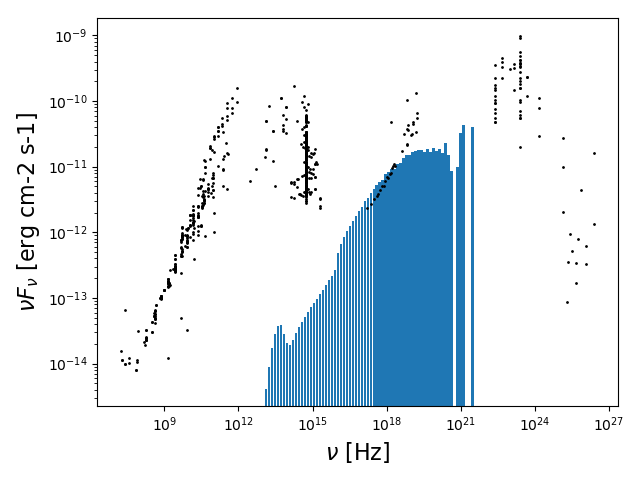
\includegraphics[width=0.8\textwidth]{3C454_3_comptSED.png}
        \caption{The SED resulting from inverse compton scattering off randomly sampled electrons for a black body distributed photon field generated at 370 Kelvin. Observational data retrieved using the ASI SSDC SED builder are indicated in black.} 
    \end{figure}
    \label{fig:comptSED}
    
    where $\alpha \approx 2.821$. In our own code we took $T=370 K$, which ought to yield similar results. Using $\Gamma=15$ for the jet lorentz bulk factor and $\alpha=\ang{6}$ for the angle between the jet and the line of sight \cite{Gupta2017}, we arrived at the spectra given in figures \ref{fig:inputSED} and \ref{fig:comptSED} for one million input photons. The underlying electron distribution given in figure \ref{fig:electron_distr} was created using a power-law index $p=2.36$ taken from \cite{Gupta2017}.

\section{Discussion and conclusion}
    Examining the different figures we were able to derive, it seems our code reproduces the spectral energy densities of 3C454.3 above $10^{18}$ Hz correctly within about one order of magnitude. However, many complications remain. Above around $10^{21}$ Hz, our SED seems limited by statistics. The probability for a randomly sampled photon and an electron to have such energies that the resulting upscattered photon will have a frequency above this value, is small and the code is not able to reproduce the appropriate spectral shape at an appreciable rate. One more huge misfit, is of course provided by the discrepancy in the optical and IR part of the SED, below $10^{15}$ Hz. In reality this part of the spectrum is not generated by black body radiation, but by synchrotron emission. To account for this part of the spectrum an attempt was made at including synchrotron within the Monte Carlo code by sampling from the characteristic single-particle synchrotron emission profile using the inversion method. However, as of yet, this didn't prove successful: SED's computed using this part of the code were not centered around the expected frequency range (i.e. around $\nu_{SSA} ~ 10^{-12} (B/\mathrm{Gauss}) (T_b / K)^2 ~ 10^{14}$ for a brightness temperature of $T_b ~ 10^{13}$ K \cite{Terasranta1994} and a magnetic field $B ~ 1$ G \cite{Gupta2017}) and moreover understimated the SED by many orders of magnitude. To make matters worse, the synchrotron code ran extremely slowly as a consequence of the expensive computational operations involved.\footnote{Sampling from the single particle synchrotron spectrum involves an integration over Bessel functions of the second kind, which is computationally very strenuous.} \\

    \par All in all, it seems our Monte Carlo code was not able to reproduce the whole SED of 3C454.3. In the frequency range between $10^[18]$ and $10^{20}$ Hz observational data is re-established fairly accurately within the range of one order of magnitude. However, above and below that, work still needs to be done. The low frequencies need to be accounted for using a properly functioning and fast-running synchrotron code, whilst the higher frequency data points may covered by taking into account an even greater number of input photons. \\
    All shortcomings aside, however, we may conclude on the note that Monte Carlo indeed forms a powerful tool for spectrum sampling. Alhtough we were not able to reproduce our entire spectrum, the general shape conforms to what one might expect (a small bump at the initial black body peak frequency around $10^13$ Hz, followed by a large hill of upscattered photons). Hence, for problems in ion transport, quantum dots and in neutrino events and graviational wave studies alike, keeping Monte Carlo in mind, might prove useful.
    



\clearpage
\section{References}
\renewcommand\refname{}
\bibliographystyle{abbrv}
\bibliography{refs.bib}





\end{document}

